%-------------------------------------------------------------------------------
% This file provides a skeleton ATLAS note.
% \pdfinclusioncopyfonts=1
% This command may be needed in order to get \ell in PDF plots to appear. Found in
% https://tex.stackexchange.com/questions/322010/pdflatex-glyph-undefined-symbols-disappear-from-included-pdf
%-------------------------------------------------------------------------------
% Specify where ATLAS LaTeX style files can be found.
\newcommand*{\ATLASLATEXPATH}{latex/}
% Use this variant if the files are in a central location, e.g. $HOME/texmf.
% \newcommand*{\ATLASLATEXPATH}{}
%-------------------------------------------------------------------------------
\documentclass[PUB,UKenglish, texlive=2018]{\ATLASLATEXPATH atlasdoc}
%coverpage=true
% The language of the document must be set: usually UKenglish or USenglish.
% british and american also work!
% Commonly used options:
%  texlive=YYYY          Specify TeX Live version (2016 is default).
%  coverpage             Create ATLAS draft cover page for collaboration circulation.
%                        See atlas-draft-cover.tex for a list of variables that should be defined.
%  cernpreprint          Create front page for a CERN preprint.
%                        See atlas-preprint-cover.tex for a list of variables that should be defined.
%  NOTE                  The document is an ATLAS note (draft).
%  PAPER                 The document is an ATLAS paper (draft).
%  CONF                  The document is a CONF note (draft).
%  PUB                   The document is a PUB note (draft).
%  BOOK                  The document is of book form, like an LOI or TDR (draft)
%  txfonts=true|false    Use txfonts rather than the default newtx
%  paper=a4|letter       Set paper size to A4 (default) or letter.

%-------------------------------------------------------------------------------
% Extra packages:
\usepackage[subfigure]{\ATLASLATEXPATH atlaspackage}
\usepackage{multirow,makecell}
% Commonly used options:
%  biblatex=true|false   Use biblatex (default) or bibtex for the bibliography.
%  backend=bibtex        Use the bibtex backend rather than biber.
%  subfigure|subfig|subcaption  to use one of these packages for figures in figures.
%  minimal               Minimal set of packages.
%  default               Standard set of packages.
%  full                  Full set of packages.
%-------------------------------------------------------------------------------
% Style file with biblatex options for ATLAS documents.
\usepackage{\ATLASLATEXPATH atlasbiblatex}

% Package for creating list of authors and contributors to the analysis.
\usepackage{\ATLASLATEXPATH atlascontribute}

% Useful macros
\usepackage{\ATLASLATEXPATH atlasphysics}
\usepackage{\ATLASLATEXPATH atlasbsm}
% See doc/atlas_physics.pdf for a list of the defined symbols.
% Default options are:
%   true:  journal, misc, particle, unit, xref
%   false: BSM, heppparticle, hepprocess, hion, jetetmiss, math, process, other, texmf
% See the package for details on the options.

% Files with references for use with biblatex.
% Note that biber gives an error if it finds empty bib files.
\addbibresource{pub-note.bib}
\addbibresource{bib/ATLAS.bib}
\addbibresource{bib/CMS.bib}
\addbibresource{bib/ConfNotes.bib}
\addbibresource{bib/PubNotes.bib}

\defbibentryset{IBL}{Capeans:1291633,CERN-LHCC-2012-009}

% Paths for figures - do not forget the / at the end of the directory name.
\graphicspath{{logos/}{figures/}}

% Add you own definitions here (file pub-note-defs.sty).
\usepackage{pub-note-defs}

%-------------------------------------------------------------------------------
% Generic document information
%-------------------------------------------------------------------------------

% Title, abstract and document 
%-------------------------------------------------------------------------------
% This file contains the title, author and abstract.
% It also contains all relevant document numbers used for an ATLAS note.
%-------------------------------------------------------------------------------

% Title
\AtlasTitle{Performance of vertex reconstruction algorithms for detection of new long-lived particle decays within the ATLAS inner detector}

% Draft version:
% Should be 1.0 for the first circulation, and 2.0 for the second circulation.
% If given, adds draft version on front page, a 'DRAFT' box on top of each other page, 
% and line numbers.
% Comment or remove in final version.
%\AtlasVersion{1.1}

% Abstract - % directly after { is important for correct indentation
\AtlasAbstract{%
Several theories beyond the Standard Model predict the existence of new particles with macroscopic lifetimes of $c\tau\gtrsim {\cal O}(1~{\rm mm})$ that could be created in $pp$ collisions at the Large Hadron Collider.
These theories often give rise to signatures requiring dedicated tracking and vertexing techniques beyond conventional algorithms.
This note presents a secondary vertex reconstruction algorithm designed to search for long-lived particles decaying within the ATLAS inner detector.
Its performance is characterised across a range of theories beyond the Standard Model with unique final states that highlight various aspects of the reconstruction.
}

% Author - this does not work with revtex (add it after \begin{document})
\author{The ATLAS Collaboration}

%\AtlasRefCode{IDTR-2019-04}
\AtlasRefCode{ATL-PHYS-PUB-2019-013}

% Authors and list of contributors to the analysis
% \AtlasAuthorContributor also adds the name to the author list
% Include package latex/atlascontribute to use this
% Use authblk package if there are multiple authors, which is included by latex/atlascontribute
% \usepackage{authblk}
% Use the following 3 lines to have all institutes on one line
% \makeatletter
% \renewcommand\AB@affilsepx{, \protect\Affilfont}
% \makeatother
% \renewcommand\Authands{, } % avoid ``. and'' for last author
% \renewcommand\Affilfont{\itshape\small} % affiliation formatting
% \AtlasAuthorContributor{First AtlasAuthorContributor}{a}{Author's contribution.}
% \AtlasAuthorContributor{Second AtlasAuthorContributor}{b}{Author's contribution.}
% \AtlasAuthorContributor{Third AtlasAuthorContributor}{a}{Author's contribution.}
% \AtlasContributor{Fourth AtlasContributor}{Contribution to the analysis.}
% \author[a]{First Author}
% \author[a]{Second Author}
% \author[b]{Third Author}
% \affil[a]{One Institution}
% \affil[b]{Another Institution}

% If a special author list should be indicated via a link use the following code:
% Include the two lines below if you do not use atlasstyle:
% \usepackage[marginal,hang]{footmisc}
% \setlength{\footnotemargin}{0.5em}
% Use the following lines in all cases:
% \usepackage{authblk}
% \author{The ATLAS Collaboration%
% \thanks{The full author list can be found at:\newline
%   \url{https://atlas.web.cern.ch/Atlas/PUBNOTES/ATL-PHYS-PUB-2016-007/authorlist.pdf}}
% }

% ATLAS reference code, to help ATLAS members to locate the paper
%\AtlasRefCode{GROUP-2016-XX}

\AtlasCoverCommentsDeadline{25 March 2019}

\AtlasCoverAnalysisTeam{Jyoti Prakash Biswal, Karri DiPetrillo, Matthew Gignac, Giuliano Gustavino, Lawrence Lee Jr, Hideyuki Oide, Jennifer Kathryn Roloff, John Stupak}

 \AtlasCoverReaderMember{Simone Pagan Griso}
 \AtlasCoverReaderMember{Philippe Mermod}

\AtlasCoverEgroupEditors{atlas-ana-idtr-2019-04-analysis-team@cern.ch}

% ATLAS note number. Can be an COM, INT, PUB or CONF note
% \AtlasNote{ATLAS-CONF-2016-XXX}
% \AtlasNote{ATL-PHYS-PUB-2016-XXX}
% \AtlasNote{ATL-COM-PHYS-2016-XXX}

% Author and title for the PDF file
\hypersetup{pdftitle={ATLAS document},pdfauthor={The ATLAS Collaboration}}

%-------------------------------------------------------------------------------
% Content
%-------------------------------------------------------------------------------
\begin{document}

\maketitle

%\tableofcontents

% List of contributors - print here or after the Bibliography.
%\PrintAtlasContribute{0.30}
%\clearpage

%%%%%%%%%%%%%%%%%%%%%%%%%%%%%%%%%%%%%%%%%%%
\section{Introduction \label{sec:intro}}
%%%%%%%%%%%%%%%%%%%%%%%%%%%%%%%%%%%%%%%%%%%

A variety of theories beyond the Standard Model (BSM) predict new particles with macroscopic lifetimes yielding a decay length of more than ${\cal O}(1~{\rm mm})$ that could be created in $pp$ collisions at the Large Hadron Collider (LHC).
Such narrow decay widths can be realised by various mechanisms, e.g.~tiny coupling constants, high virtuality of the intermediate propagator to the decay, compression of the BSM mass spectrum, etc. 
%Analogous mechanisms are present in the Standard Model (SM) hadrons or leptons with macroscopic lifetimes.
If the decay of such hypothetical long-lived particles (LLPs) to Standard Model (SM) charged hadrons or leptons takes place within the inner tracking volume of the ATLAS detector\footnote{ATLAS uses a right-handed coordinate system with its origin at the nominal interaction point (IP) in the centre of the detector and the $z$-axis along the beam pipe. 
The $x$-axis points from the IP to the centre of the LHC ring, and the $y$-axis points upward. Cylindrical coordinates $(r, \phi)$ are used in the transverse plane, $\phi$ being the azimuthal angle around the $z$-axis. 
The pseudorapidity is defined in terms of the polar angle $\theta$ as $\eta = -\ln(\tan(\theta/2))$, and angular distance is measured in units of $\Delta R \equiv \sqrt{(\Delta\eta)^{2} + (\Delta\phi)^{2}}$.}, it can be identified using outgoing tracks from a vertex significantly displaced from the primary $pp$ interaction. 
Despite the harsh pileup collision conditions of the LHC, 
such secondary vertices can offer a highly-distinctive signature for BSM searches.

Tracks corresponding to outgoing charged particles from decays of such hypothetical LLPs could have relatively large transverse and longitudinal impact parameters\footnote{The transverse impact parameter $d_{0}$
is defined as the distance of closest approach in the transverse plane between a track and the beam-line. The longitudinal impact parameter $z_{0}$ corresponds to the $z$-coordinate distance between the point 
along the track at which the transverse impact parameter is defined and the primary vertex.} of more than tens of millimetres, depending on the decay position. Such tracks are collectively referred to as \emph{large-radius  tracks}.
The standard ATLAS track reconstruction, which is not optimised for such particles, limits the transverse (longitudinal) impact parameter range to $\pm10~{\rm mm}$ ($\pm250~{\rm mm}$) within the nominal interaction point.
The reconstruction efficiency for large-radius tracks can be then recovered with an additional specialised tracking configuration, referred to as the large-radius tracking~\cite{ATL-PHYS-PUB-2017-014}. 
Due to significantly larger computing cost and data size, it can only be applied to a specially selected dataset for LLP searches, filtered from the main physics dataset. 
Reconstruction of secondary vertices are based on this extended track reconstruction.

Several reconstruction algorithms targeting vertices with significant displacement from the primary $pp$ interactions, collectively referred to as \emph{secondary vertex} reconstructions, exist for various applications in ATLAS. 
The vertex reconstruction algorithm studied in this article is based on the one used in the inner tracker material study using hadronic interactions~\cite{ATLAS-CONF-2010-058,Aaboud:2016poq,Aaboud:2017pjd} 
as well as preceding BSM searches~\cite{Aaboud:2017iio,Aad:2015rba,Aad:2011zb,Aad:2012zx}, but the algorithm has been modified to improve performance for searches using the full Run~2 dataset.

% M.G.
%Aad:2015uaa --> Used an adapted PV finding algorithm. Removing this one.



%%%%%%%%%%%%%%%%%%%%%%%%%%%%%%%%%%%%%%%%%%%
\section{ATLAS inner detector}
%%%%%%%%%%%%%%%%%%%%%%%%%%%%%%%%%%%%%%%%%%%


The ATLAS inner detector is a cylindrical tracking system immersed in a 2~T axial magnetic field covering $|\eta|<2.5$. 
It comprises three different technologies of silicon pixel, silicon micro-strip (SCT) and straw drift tube transition radiation tracker (TRT) detectors.

The pixel detector has four barrel layers at radii of $33, 50.5, 88.5$, and 122.5~mm and three disks in each of the end-caps at $|z|=495, 580$, and 650~mm. 
The innermost barrel layer of the pixel detector, referred to as the insertable $b$-layer (IBL)~\cite{IBL,Abbott:2018ikt}, was installed in 2014, complementing the existing pixel layers. 
In each pixel barrel layer, pixel modules are mounted on staves which run along the $z$-direction, and the staves are arrayed cylindrically with small partial overlap between contiguous staves (for hermiticity).  %arrayed with tilt angles of $11^{\circ}\hbox{--}14^{\circ}$ and small partial overlap between contiguous staves for hermiticity. 
The standard pixel size is $50~{\rm \mu m}~(r\hbox{--}\phi)\times250~{\rm \mu m}~(z)$ for IBL and $50~{\rm \mu m}~(r\hbox{--}\phi)\times400~{\rm \mu m}~(z)$ for the outer barrel and disk layers, except edge pixels. 
The coverage of the stave in $z$ is approximately $\pm300~{\rm mm}$ for IBL and $\pm400~{\rm mm}$ for the outer layers. The disk layers complement the overall pseudorapidity coverage for the range $|\eta|\gtrsim2$. 
%Charge deposited in each pixel is measured in terms of the time-over-threshold of the pulse and recorded with either 4-bit precision in the case of the IBL, or 8-bit precision in the other layers. 
%Contiguous pixel hits are grouped as clusters, and the charge-weighted centroid of each cluster is calculated for better estimating the hit position of the track. 
%For dense environment e.g.~in hadronic jet cores, a neural network trained for the cluster shape and charges further provides suggestions if a cluster likely originates from simultaneous injection of multiple particles, and it is used for optimisation of track ambiguity resolving algorithm~\cite{PERF-2015-08}.

The SCT has four barrel layers at radii of $299, 371, 443,~{\rm and}~514~{\rm mm}$, spanning $|z|<746~{\rm mm}$, and nine wheels in each of the end-caps with $854~\mathrm{mm}<|z|<2720$~mm. %covering approximately $1.2 < |\eta| < 2.5$. 
Each strip has a $80~{\rm \mu m}$ pitch and 128~mm length running approximately along the $z$- ($r$-) direction for the barrel (end-caps). 
%with contiguous modules partially overlapping to ensure hermiticity.  
Each module consists of a double-sided sensor with a stereo angle of $40~{\rm mrad}$, providing nominally a pair of measurements per layer.
Combined measurements from each sensor on a layer provide a three-dimensional position measurement referred to as a space-point. 
Measurements in each side of a module are counted as individual hits.
%The SCT only records binary information of hits. Hits of each side of a sensor plane are counted individually, meaning that tracks traversing the entire SCT barrel layers should generally produce eight SCT hits.

Beyond the silicon trackers, the outer volumes of the inner detector are furnished with the TRT. 
It is comprised of approximately 300\,000 straw tubes and covers the pseudorapidity range of $|\eta|<2$ with a radial extension to $r<1066~{\rm mm}$.
Each straw tube only provides two-dimensional position information with position resolution of approximately $130~{\rm \mu m}$. 
Straw tubes in the barrel region  ($|z|< 712~{\rm mm}$) run along the $z$-direction providing $(r,\phi)$ information, while for end-caps ($848~\mathrm{mm}<|z|<2710~\mathrm{mm}$) they run in the radial direction providing $(z,\phi)$ information.

%%%%%%%%%%%%%%%%%%%%%%%%%%%%%%%%%%%%%%%%%%%
\section{Large-radius tracking}
%%%%%%%%%%%%%%%%%%%%%%%%%%%%%%%%%%%%%%%%%%%

The standard ATLAS track reconstruction has been optimised and designed primarily to reconstruct tracks originating from the primary $pp$ collision region (though some capability exists to reconstruct tracks originating from displaced locations, such as high-$p_T$ photon conversions).
As such, it imposes tight upper bounds on the transverse and longitudinal impact parameter for all tracks.
Particles emitted from a long-lived particle decaying within the inner detector can have large impact parameters relative to the primary $pp$ collision point, 
and are not efficiently reconstructed by the standard track reconstruction.
In order to recover these tracks, an additional large-radius tracking (LRT)~\cite{ATL-PHYS-PUB-2017-014} configuration is performed with relaxed impact parameter requirements.

The LRT configuration runs after the standard track reconstruction using only hits not already associated to tracks from the standard reconstruction pass. 
This configuration requires reconstructed tracks to have a minimum of seven silicon hits (pixel or SCT). 
The largest reconstructible decay radius ($r_{\rm vtx}$) is nominally around $300~{\rm mm}$, corresponding to the innermost SCT barrel layer. In order to reconstruct tracks from particles produced at such large radii, the transverse impact parameter requirement is relaxed to $|d_{0}|<300~{\rm mm}$.  The longitudinal impact parameter requirement is similarly relaxed to $|z_{0}|<1500~{\rm mm}$. %, to be consistent with the above situation. 
The minimum transverse momentum $\pt$ is raised to 900~\MeV~instead of 500~\MeV~as in the case of Ref.~\cite{ATL-PHYS-PUB-2017-014} to mitigate efficiency losses due to high pileup conditions. 

%%%%%%%%%%%%%%%%%%%%%%%%%%%%%%%%%%%%%%%%%%%
\section{Vertex reconstruction}
%%%%%%%%%%%%%%%%%%%%%%%%%%%%%%%%%%%%%%%%%%%

Secondary vertex reconstruction is seeded by pairs of tracks which are roughly compatible with production from a long-lived particle decay.  
Due to the high multiplicity of tracks in typical LHC collisions, it is not feasible to consider all possible pairs of tracks.  
Instead, tracks are preselected for vertex seeding with a series of quality criteria.  
The compatibility of each possible pair of preselected tracks is assessed, and those deemed loosely compatible are retained.  
These two-track seed vertices are then combined to form multi-track vertices through the use of an incompatibility graph.  
Nearby vertices are then merged, and lower-quality tracks not initially preselected for vertex seeding are attached to compatible vertices. 

Unlike other secondary vertexing algorithms, including the jet-seeded one used for $b$-tagging~\cite{Aad:2015ydr,ATL-PHYS-PUB-2017-011}, 
the algorithm studied here imposes no specific restrictions on the input track collection in terms of track orientation, 
and therefore it can potentially reconstruct a wide phase space of outgoing track combinations throughout the inner detector.
The algorithm is designed to be highly-configurable for potential uses beyond those described in this note, and the performance can depend on those configuration parameters. 
The performance in Section~\ref{sec:performance} is evaluated using the parameters described in the remainder of this section.

% We are not using the lepton configuration; shows issues...
%In this note, two reconstruction configuration options are used and the performance results are reported with respect to these options: 
%the first one is the \emph{inclusive} configuration. In this configuration, the inner detector tracks are selected for seeding solely based on the individual track parameters. 
%The second configuration is the \emph{leptonic} configuration, where the tracks associated to reconstructed electron or muon objects are used for seeding, without 
%any other selections, in an effort to obtain high reconstruction efficiencies for displaced leptonic vertices. 
%The sparsity of leptons in typical events allows such reconstruction with a relatively low computing cost.

%%%%%%%%%%%%%%%%%%%%%%%%%%%%%%%%%%%%%%%%%%%
\subsection{Seed track selection \label{sec:vtxReco:trackSelection} }
%%%%%%%%%%%%%%%%%%%%%%%%%%%%%%%%%%%%%%%%%%%

Tracks are preselected for the formation of seed vertices. The selection is designed to be as inclusive as possible to allow an efficient reconstruction of secondary vertices across a wide range of models.
Tracks reconstructed by the standard and LRT configurations are used throughout the vertex reconstruction.

All tracks are required to have transverse momentum $\pt>1~\GeV$. Tracks are explicitly required to not be associated to any primary vertex (from the hard-scatter or pileup interactions)~\cite{Aaboud:2016rmg}. Tracks are further required to satisfy the following criteria in order to reject low-quality tracks:
\begin{itemize}
\item if the track has zero associated pixel hits, it must have at least six associated hits in the SCT;
\item if the track has fewer than two associated pixel hits, it must have at least one associated hit in the TRT;
\item if the track $\pt$ is less than $20~\GeV$, it must have at least seven associated hits in the SCT. In addition, if the track $|\eta|$ is less than 1.7, it must have at least 20 associated hits in the TRT.
\end{itemize}


%%%%%%%%%%%%%%%%%%%%%%%%%%%%%%%%%%%%%%%%%%%
\subsection{Two-track seed finding}
%%%%%%%%%%%%%%%%%%%%%%%%%%%%%%%%%%%%%%%%%%%

The vertex finding starts by forming all possible pairs of preselected tracks with $|d_{0}|>2~{\rm mm}$. 
For each pair, a fast calculation is used to determine an approximate vertex position using the track parameters measured at the perigee\footnote{The perigee is the point of closest approach to the beam spot}. 
For pairs in which both tracks have small impact parameters with respect to this position, an accurate track extrapolation is performed
and the vertex candidate is discarded if the fitting algorithm~\cite{Kostyukhin:2003daa} cannot find a viable solution. 
This fitting algorithm minimises the $\chi^{2}$ of the vertex ($\chi^{2}_{\mathrm{vtx}}$), which penalises large differences of the track parameters with respect to the vertex position weighted by the covariance of the track parameters.
All tracks are taken with equal weights.
The minimisation is implemented in a Kalman filter system, taking one-by-one addition of constituent tracks to the $\chi^{2}_{\mathrm{vtx}}$ as the incrementing step of the filter. 
The number of degree of freedom, $n_{\mathrm{dof}}$ is $2n-3$ where $n$ is the number of constituent tracks. 
If a solution is found but $r_{\rm vtx}$ is greater than $563~{\rm mm}$ (corresponding to the SCT/TRT boundary) or the reduced vertex-fitting quality, $\chi^{2}_{\rm vtx}/n_{\rm dof}$, is greater than $5$, the vertex candidate is rejected.

Both tracks composing the vertex candidate are then required to fulfil the so-called ``hit-pattern consistency.''  % is required for the seed tracks, assuming that they originate from the vertex. 
The concept of this requirement is that the tracks should have hits in tracker layers with radii beyond the vertex candidate position, and should not have hits in tracker layers with radii smaller than the vertex candidate position %layers 
(tracks typically travel outwards through the tracker), as illustrated in Figure~\ref{fig:fakeRejScheme}. 
% TODO: What does fairly close to sensor layers mean? Can we be a bit more qualitative??
% https://gitlab.cern.ch/atlas/athena/blob/21.0/Reconstruction/VKalVrt/VrtSecInclusive/src/Utilities.cxx#L1431-1472
This requirement is not enforced for tracker layers in close proximity to the vertex candidate position, to accommodate vertex position mis-measurement.  %When the seed vertex position is close to a tracker layer. %relaxed to allow ambiguity of having or missing hits at the closest layer. 
Vertex candidates where both tracks fulfil this hit-pattern consistency are retained. 
Temporarily or permanently disabled silicon modules do not produce hits, and tracks traversing such modules would not nominally satisfy the hit-pattern consistency. 
In order to remedy this, %the condition of activeness of modules are queried, and the layers with disabled modules are treated as if they would have hits on the module. 
tracker layers with disabled modules are treated as if they had indeed produced a hit, thereby improving the reconstruction efficiency of the vertices near disabled modules. 
%This additional treatment improves the reconstruction efficiency of the vertices nearby disabled modules.

\begin{figure}[t]
\begin{center}
\subfigure[]{ 
  \label{fig:HadInt:fakeRejScheme1} 
  \includegraphics[width=0.45\textwidth]{figures/fakeRejectionScheme1}
}
\subfigure[]{ 
  \label{fig:HadInt:fakeRejScheme2} 
  \includegraphics[width=0.45\textwidth]{figures/fakeRejectionScheme2}
}
\caption{The schematic shows as example a transverse view of the pixel detector in the barrel region. \subref{fig:HadInt:fakeRejScheme1} 
The vertex is between the two layers of B-Layer and Layer-1 sensors.
The tracks of the reconstructed secondary vertex must not have hits on the layers within the vertex radius (i.e.~IBL and B-Layer), 
and must have hits on the closest layer outside the vertex (i.e.~Layer-1). 
\subref{fig:HadInt:fakeRejScheme2} The vertex is close to the pixel B-Layer sensors. 
In this example where the vertex is inside the B-Layer, 
the tracks are not allowed to have hits on the IBL but may have hits on the B-Layer, and must have hits on the Layer-1. 
Analogous requirements are made on vertices close to the other layers.
}
\label{fig:fakeRejScheme}
\end{center}
%\end{figure}

%\begin{figure}[t]
\begin{center}
\subfigure[]{ 
  \label{fig:graph1} 
  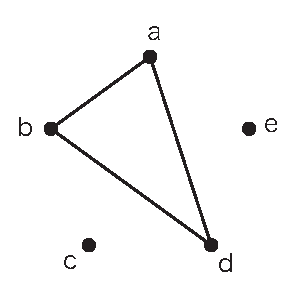
\includegraphics[width=0.18\textwidth]{figures/graph1}
}
\hspace{2cm}
\subfigure[]{ 
  \label{fig:graph2} 
  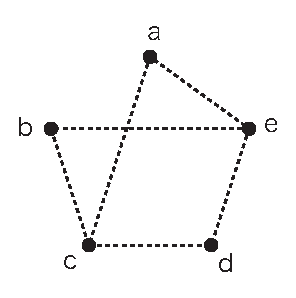
\includegraphics[width=0.18\textwidth]{figures/graph2}
}
\caption{Illustration of (in)compatibility graph for a five-nodes (tracks) case where three tracks $(a,b,d)$ form a common vertex. 
\subref{fig:graph1} the nodes $(a,b,d)$ are compatible each other (the compatibility graph). 
\subref{fig:graph2} the same state can also be expressed by connecting incompatible nodes (the incompatibility graph). 
Removing the nodes $c$ and $e$ (and all associated dotted edges from them) makes the nodes $(a,b,d)$ all isolated, meaning that these three nodes are compatible each other.}
\label{fig:incompGraph}
\end{center}
\end{figure}

%%%%%%%%%%%%%%%%%%%%%%%%%%%%%%%%%%%%%%%%%%%
\subsection{Multi-track vertex forming}
%%%%%%%%%%%%%%%%%%%%%%%%%%%%%%%%%%%%%%%%%%%

During the two-track vertex finding stage, tracks originating from a common LLP decay can be used to form multiple two-track seed vertices,
or a single track can be used multiple times in different seed vertices.
In order to form multi-track vertices, the state of all paired tracks is modeled using an undirected graph network by mapping tracks as nodes and two-track vertices as edges. 
%A reconstructed vertex with $n$ constituent tracks has $C(n,2)$ track pair combinations,  pointing to a similar vertex position at the two-track vertex finding step. 
%The state of paired tracks by two-track vertex finding can be modelled using an undirected graph network by mapping tracks as nodes and two-track vertices as edges. 
Such a graph is referred to as a compatibility graph (the nodes connected by edges are referred to as \emph{compatible}.) 
The same state can be equivalently modelled by connecting the nodes which do not form vertices, referred to as an \emph{incompatibility graph}, as illustrated in Figure~\ref{fig:incompGraph}. 
A group of nodes which are fully compatible with each other can be extracted by removing all irrelevant nodes from the incompatibility graph\footnote{This calculation is possible to perform efficiently using a classic algorithm originally implemented in CERNLib {\texttt V401}.}. 
The extracted group of tracks are simultaneously fitted as a single multi-track vertex. 
% Dropping this line as it's no longer used: https://gitlab.cern.ch/atlas/athena/blob/21.0/Reconstruction/VKalVrt/VrtSecInclusive/src/Utilities.cxx#L263
%The goodness of fitting as well as goodness of association of each track to the vertex is evaluated, and badly associated tracks are dropped.

At this point, a single track can be still associated to different vertices which are significantly displaced from each other. 
Since the algorithm only allows for a given track to be associated to a single secondary vertex, 
the goodness of association to these vertices sharing the same track is evaluated, and only the association to the best-fitting vertex is kept.

%%%%%%%%%%%%%%%%%%%%%%%%%%%%%%%%%%%%%%%%%%%
\subsection{Vertex merging}
%%%%%%%%%%%%%%%%%%%%%%%%%%%%%%%%%%%%%%%%%%%

Multiple secondary vertices corresponding to a single LLP decay can be reconstructed by the above algorithm. Such a state is referred to as \emph{split}. Split vertices result in a deterioration of the vertex track multiplicity and invariant mass.  
This is not preferable for discrimination of a BSM signature using these quantities. In order to mitigate splitting, nearby vertices are allowed to be merged into a single vertex. 

Candidates for vertex merging are chosen in ascending order of selected track multiplicity. 
The algorithm attempts to merge each candidate with all other vertices with higher selected track multiplicity, in descending order of selected track multiplicity. 
In the following, the lower selected track multiplicity vertex will be denoted ``LMV,'' while the higher selected track multiplicity vertex will be denoted ``HMV.''

In the procedures below, vertices are considered compatible with each other and merged if the two positions are within 10$\sigma$,
where $\sigma$ is the uncertainty on the difference between the two vertex positions,
calculated as the quadrature sum of the covariance matrices of the two individual vertex fits.  
Three separate tests are used to determine if two vertices should be merged into a single vertex:

\begin{itemize}
\item{Vertices with a larger number of tracks have an improved position resolution compared to those with a smaller number of tracks~(see Section~\ref{sec:position_resolution}).
         In order to address the situation that the LMV originates from the HMV but is distinguished from the HMV due to its poor position resolution, the LMV is seeded with the position of the HMV and refit. 
         The vertices are merged and refit as a single vertex if the updated vertex position is compatible with the HMV position.}
\item{The selected tracks associated to the HMV are iteratively associated to the LMV and the vertex is refit, again seeded by the position of the HMV. 
         If any of the refit vertices are compatible with HMV vertex position they are merged and refit as a single vertex.}
\item{All of the selected tracks from both vertices are used in a single vertex fit using the position of the HMV to seed the vertex fit.  
         If the refit vertex is compatible with the HMV position, the vertices are merged and refit as a single vertex.}
\end{itemize}

The above thresholds are tuned to minimise the number of split vertices, while accepting a small fraction of accidental merging of unrelated vertices. 
Any remaining vertices within 1~mm are forced to merge, and all merged vertices are refit with all tracks from the two input vertices.

%%%%%%%%%%%%%%%%%%%%%%%%%%%%%%%%%%%%%%%%%%%
\subsection{Track attachment}
\label{sec:attachment}
%%%%%%%%%%%%%%%%%%%%%%%%%%%%%%%%%%%%%%%%%%%

At this point, only selected seed tracks contribute to the vertex reconstruction, but there could be reconstructed tracks that originate from the vertex that do not satisfy the seed track selection criteria.
Association of such tracks to the reconstructed vertex can improve certain vertex kinematics properties  (e.g.~track multiplicity and invariant mass).
Impact parameters with respect to the secondary vertex are calculated for all unused reconstructed tracks satisfying $\pt>1~{\rm GeV}$ and the track $\chi^{2}/n_{\rm dof}<5$. This includes tracks which are already associated to primary $pp$ interactions.
Tracks with transverse and longitudinal impact parameter significances with respect to the target secondary vertex less than 5 are selected to be associated to the vertex. 
A relaxed hit-pattern consistency of only checking the presence of the hits in the outer layers is required to potentially accept back-scattered tracks which might not fulfil the inner layer hit pattern. 
A track is limited to only be associated to a single secondary vertex, and this attempt is made in the descending order of the track multiplicity of the vertex. Tracks already associated to any secondary vertex are not considered for further association to other vertices. 
The vertex position is re-fit for each attempted track association. Attachment is not accepted if $\chi^{2}_{\rm vtx}/n_{\rm dof}$ is greater than 20. 
This track attachment procedure is designed to accept as many tracks as possible with a loose requirement applied during reconstruction where track parameter extrapolation and vertex re-fitting is available. 
Such tracks may be subject to pruning at the analysis stage, since the optimal criteria are likely analysis specific.

At this point, a final fit is performed (including all of the tracks which were successfully attached) and track parameters with respect to the vertex position are re-calculated. 
The nominal vertex invariant mass is calculated assuming the charged pion mass for all tracks, using the track momentum vectors at the location of the vertex.

%%%%%%%%%%%%%%%%%%%%%%%%%%%%%%%%%%%%%%%%%%%
\section{Simulated event samples \label{sec:Dataset} }
%%%%%%%%%%%%%%%%%%%%%%%%%%%%%%%%%%%%%%%%%%%

%TODO: We need to add in details of their generator setup, reconstruction configuration, etc

The performance of the secondary vertex reconstruction is evaluated using three representative benchmark decay classes of hypothetical LLPs. 
The following models are considered: 

%
% Summary of the models
%
\begin{itemize}

\item The first benchmark model probes the performance for LLP decays producing high-multiplicity hadronic secondary vertices. It is a supersymmetric model that assumes the neutralino is the lightest supersymmetric particle that is produced during the cascade decay of a heavier gluino particle, $pp\rightarrow\gluino\gluino,~\gluino\rightarrow qq\ninoone~(q=u,d,s,c)$, where the $\ninoone$ decays to light quarks $\ninoone\rightarrow qqq$ via off-shell first and second generation squarks, as shown in Figure~\ref{fig:models:gluino}.
The mass of the squarks and gluino are 3 and 2.4~TeV respectively.  For the bulk of the studies presented in this note, the neutralino mass is 2050~GeV, but the mass range 50--2350~\GeV\ is considered in Section~\ref{sec:vertProp}.  The mean proper lifetime of the neutralino is controlled by the size of the $\lambda''_{112}$ $R$-parity-violating coupling \cite{FARRAR1978575,HALL1984419,ROSS1985375,PhysRevD.40.2987,doi:10.1142/9789814307505_0017,PhysRevD.69.115002}, and set to $300~{\rm mm}/c$.
%The $\ninoone$ lifetime is controlled by the size of the $\lambda''_{112}$ $R$-parity-violating coupling \cite{FARRAR1978575,HALL1984419,ROSS1985375,PhysRevD.40.2987,doi:10.1142/9789814307505_0017,BARBIER20051,PhysRevD.69.115002}.
Signal samples were generated at leading-order (LO) accuracy with up to two additional partons in the matrix element using the \textsc{MadGraph}5\_aMC@NLO v2.3.3 event generator~\cite{Alwall2014} 
interfaced with \textsc{Pythia} 8.212~\cite{Sjostrand:2014zea}, using the A14~\cite{ATL-PHYS-PUB-2014-021} tune for the underlying event. 
The parton luminosities are provided by the NNPDF2.3LO~\cite{Ball:2014uwa} PDF set.
%The benchmark models explored in this note assume a gluino mass of $m(\gluino)$~=~2400~GeV, and a neutralino mass, $m(\ninoone)$, ranges from 10~\GeV~to 2350~\GeV~with a proper lifetime of $\tau=1$~ns.


\item{Inspired by hidden-sector models with a Higgs portal~\cite{Strassler:2006im,Schabinger:2005ei,Patt:2006fw}, we consider the production of the SM Higgs boson in association with a $W^{\pm}$ boson, 
with the Higgs boson decaying to a pair of BSM pseudoscalar bosons $a$, as shown in Figure~\ref{fig:models:VH}.  
In such models, the $a$~boson generally decays through an off-shell Higgs boson, and therefore inherits Yukawa (effective) couplings to SM fermions and obtains a long lifetime.  
As a result, we consider decays of the $a$~boson to pairs of bottom quarks.  In this model, the pseudoscalar boson has a mass $m(a)=55$~GeV and mean proper lifetime $\tau=100~{\rm mm}/c$.
%For $a$ boson masses $m_a > 2m_b$, the $a$ decays preferentially to pairs of bottom quarks.  Therefore, we assume $BR(a\rightarrow b\overline{b})=1$.  
Due to the $B$~hadron lifetime and subsequent decay chain, a single $a$~boson can give rise to multiple vertices.  
Although the algorithm was not optimised to separately reconstruct such nearby vertices, in some cases this will occur.  
In order to highlight the effects of the non-negligible $B$~hadron lifetime, we also compare this model to one where  the $a$~boson decays to pairs of up quarks.
Events were generated at next-to-leading-order (NLO) accuracy with up to one extra parton in the matrix element using the \textsc{Powheg}~\cite{Frixione:2007nw,Nason:2004rx} event generator
interfaced to \textsc{Pythia} 8.212 for the decay of the Higgs boson and parton showering.
%The benchmark model explored in this note for this model assumes as mass of the pseudoscalar boson $m(a)=55$~GeV with proper lifetime $\tau=100~{\rm mm}/c$.
}
 
\item{The existence of three heavy, right-handed neutrinos could potentially explain the origin of neutrino mass, the baryon asymmetry, and dark matter~\cite{Asaka:2005pn,Canetti:2012vf}.  This requires the heavy neutral leptons (HNLs), $N$, to have small mixing with the light neutrinos.  As a result, the HNLs would have long lifetimes.  %Here, we consider fully-leptonic decays, $N\rightarrow\nu_{\ell}\ell^{\pm}\ell^{\prime\mp}$, as shown in Figure~\ref{fig:models:HNL}.  
This signature provides a convenient means to assess the performance of the algorithm for low-track-multiplicity secondary vertices by considering decays of the HNL to $\nu_{\mu}\mu^{+}\mu^{-}$, as shown in Figure~\ref{fig:models:HNL}.  In this model, the heavy neutral lepton has a mass $m(N)=15$~GeV and mean proper lifetime $\tau=100~{\rm mm}/c$.  
Events are generated using \textsc{Pythia} 8.212, using the NNPDF2.3LO PDF set and the A14 set of tuned parameters.}
\end{itemize}

All signal Monte Carlo (MC) samples are overlaid with simulated minimum-bias events to model the effects of multiple interactions per bunch crossing. 
The average number of $pp$ interactions is chosen to match the data taking conditions in 2017 and ranges between 10 and 80 $pp$ interactions in a given bunch crossing.
The response of the tracking detector to particles is modelled using {\texttt Geant4}~\cite{AGOSTINELLI2003250}.

The benchmark models with the masses and lifetimes considered in this note are summarised in Table~\ref{tab:benchmark_models}.

\begin{table}[htbp]
\caption{Benchmark models used for the evaluation of the secondary vertex reconstruction performance. }
\centering
\footnotesize
\begin{tabular}{cclp{1.2cm}p{1.1cm}cp{2cm}}
\toprule
Process & LLP & Secondary vertex type & LLP mass [\GeV] & LLP mean proper lifetime [${\rm mm}/c$] & Other params. \\
\midrule
%\multirowcell{3}{$pp\rightarrow\gluino\gluino$,~~$\gluino\rightarrow qq{\ninoone}$,\\${\ninoone}\rightarrow qqq$} & \multirow{3}{*}{\ninoone} &\multirow{3}{*}{hadronic (light flavor)} &  2050 & 1.0 & \multirow{3}{*}{$m(\gluino) = 2400~\GeV$} \\
%& & & 1250 & 1.0 & \\
%& & & 50 & 0.1 &\\
$pp\rightarrow\gluino\gluino,~\gluino\rightarrow qq{\ninoone}, {\ninoone}\rightarrow qqq$ & \ninoone & hadronic (light flavor) & 50--2350 & 300 & $m(\gluino) = 2400~\GeV$ \\
\midrule
 $pp\rightarrow W^{\pm}h,~~h\rightarrow aa,~~a\rightarrow bb/uu$ & $a$ & hadronic (heavy and light flavour) &  55 & 100 & \\
\midrule
%\multirowcell{2}{$pp\rightarrow W^{\pm}\rightarrow \ell^{\pm} N,~~N\rightarrow \ell^{\pm}\nu'\ell'^{\mp}$} & \multirow{2}{*}{$N$} &\multirow{2}{*}{leptonic} & 10 & $\mathcal{O}(0.01)$ & \\
$pp\rightarrow W^{\pm}\rightarrow \ell^{\pm} N,~~N\rightarrow \ell^{\pm}\nu'\ell'^{\mp}$ & $N$ & leptonic & 15 & 100 &  \\
\bottomrule
\end{tabular}
\label{tab:benchmark_models}
\end{table}%

\begin{figure}[h]
\begin{center}
% Gluino model
\subfigure[Long-lived neutralino]{ 
  \label{fig:models:gluino} 
  \includegraphics[width=0.3\textwidth]{figures/gluinoModel}
}
% Vh model
\subfigure[Higgs portal]{ 
  \label{fig:models:VH} 
  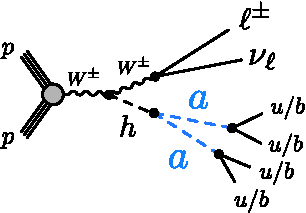
\includegraphics[width=0.3\textwidth]{figures/VHaa_new}
}
% HNL model
\subfigure[Heavy neutral lepton]{ 
  \label{fig:models:HNL} 
  \includegraphics[width=0.35\textwidth]{figures/HNL_new}
}
\caption{Representative Feynman graphs of models used to characterise the performance of the vertexing algorithm.}
\label{fig:feyModels}
\end{center}
\end{figure}



%%%%%%%%%%%%%%%%%%%%%%%%%%%%%%%%%%%%%%%%%%%
\section{Performance}\label{sec:performance}
%%%%%%%%%%%%%%%%%%%%%%%%%%%%%%%%%%%%%%%%%%%

The performance of the vertexing algorithm is evaluated using the benchmark models discussed in Section~\ref{sec:Dataset}. 
Reconstructed vertices are associated to vertices in the MC event record and the efficiency of reconstructing a given generator-level (truth) vertex is assessed.
The procedure for matching truth to reconstructed vertices is described in Section~\ref{sec:truthMatching}, and the resulting efficiency is defined in Section~\ref{sec:effDef}.
Additional studies on the the properties of the reconstructed vertices are studied in later sections, such as the vertex position resolution in Section~\ref{sec:position_resolution} and the rate of vertex splitting in Section~\ref{sec:vtx_splitRate}.

%%%%%%%%%%%%%%%%%%%%%%%%%%%%%%%%%%%%%%%%%%%
\subsection{Truth matching \label{sec:truthMatching} }
%%%%%%%%%%%%%%%%%%%%%%%%%%%%%%%%%%%%%%%%%%%

In this study, it is necessary to associate the reconstructed vertices to LLP decays in order to evaluate the performance of reconstruction efficiency. 
One simple possible approach would be to ask for the relative distance between the LLP decay position and the vertex position, 
but this attempt does not provide an inclusive evaluation especially when the LLP decay products contain short-lived particles like heavy-flavour mesons. 
Given that the main interest of the algorithm for search analyses is not the precision of the reconstruction position but tagging the presence of the LLP decay,
it is more effective to ask for the purity of the reconstructed vertices by the LLP decay, i.e.~how often the reconstructed vertex is occupied by tracks which are corresponding to the descendent particles of the LLP decay.

With the above concept, in this study LLP decays are considered as reconstructed if a vertex is found whose constituent tracks are primarily matched to truth particles produced (either directly or indirectly through a cascade) from the LLP decay. 
A truth-vertex matching score $s$, which uses the magnitude of the track $\pt$ as a weight, is defined for an arbitrary pair of a reconstructed vertex $v$ and an LLP decay $l$ as follows:
\begin{equation}
\label{eq:matchScore}
s(v,l) \equiv \frac{\displaystyle \sum_{i\,\in\,{\rm tracks}\in~v} \left(\pt^{(i)}~|~{\rm descendent~of~LLP~decay}~l\right)}{\displaystyle \sum_{i\,\in\,{\rm tracks}\in~v}\pt^{(i)}}~~.
\end{equation}
The sum in the denominator extends over all tracks in the reconstructed vertex, while the sum in the numerator extends only over those matched to truth particles from the LLP decay.  
The matching of tracks to truth particles is based on a weighted scoring of shared detector hits between the track and truth particle trajectories.

The match score can take values in the range $[0,1]$.  For $s(v,l)=1$, all of the tracks forming the reconstructed vertex are matched to truth particles produced in the decay of the LLP; for $s(v,l)<1$, there is some contamination of the reconstructed vertex by fake tracks or tracks not produced in the decay of the LLP; for $s(v,l)=0$, none of the tracks forming the reconstructed vertex are matched to truth particles produced in the decay of the LLP. 

LLP decays are regarded as reconstructed if a vertex has an associated match score greater than 0.5. This provides the basis of efficiency evaluation discussed in the next section. 
Figure~\ref{fig:match_score} shows the distribution of $s(v,l)$ for reconstructed vertices satisfying $s(v,l)>0$. As presented, the majority of reconstructed vertices satisfy this requirement and generally have scores close to unity, indicating a high purity of tracks resulting from the associated LLP decay. %If any of the truth vertex positions within the 10~mm distance from the LLP decay is reconstructed, such an LLP decay is also regarded as reconstructed. 

%Unstable hadronic LLP daughters which decay through the strong interaction will yield stable daughter particles which are effectively prompt with respect to the LLP decay vertex, but these are nominally recorded as different truth vertex instances pointing the same physical position. It is therefore natural to group the decay products from these hadrons as a part of the outgoing stable particles originating from the LLP decay itself. 
%%Products of the LLP decays via strong interactions are almost prompt from the LLP decay, and it is natural to include the decay products from these hadrons as a part of the outgoing stable particles originating from the LLP decay. 
%If unstable LLP daughters travel a relatively short distance before decaying, like heavy-flavour hadrons, the decay products from these short-lived particles may yield distinct tertiary vertices, or the tertiary vertices may be indistinguishable from the LLP decay vertex.  Therefore, one LLP decay would have a chain of multiple truth vertex positions corresponding to these cascade decays of descendants. For search analyses under consideration, it is not primarily important to which truth positions of these LLP decay cascades the reconstructed vertex is most strongly associated, but it is sufficient to identify if the reconstructed vertex is associated to the LLP decay cascade. Meanwhile, each track can have a corresponding truth charged particle that are matched based on scoring using hits, and each truth particle has a production position. If the majority of the constituent tracks of the reconstructed vertex share the same truth production position via the matched truth particles, these reconstructed vertex and the truth vertex position are regarded as matched.
%%mix in the vertex reconstruction of the LLP decay position, or they may form a separate vertex near the LLP decay point. 
%%However, for most of the applications of this DV reconstruction algorithm, it is advantageous to reconstruct a single high-mass, high-multiplicity DV rather than multiple low-mass, low-multiplicity DVs.  Therefore, the algorithm is prioritised to merge nearby reconstructed DVs than resolving them, and the truth-matching strategy should be coherent with this design. %it does not need to differentiate this detail and rather important discriminants in the search are the multiplicity and the invariant mass.
%%As such, it is reasonable to also consider stable particles from short-lived descendants of the LLP. %, instead of excluding them. 
%
%In order to seek truth vertex positions in the LLP decay cascade, firstly truth particles satisfying the following conditions are counted as potentially reconstructible particles from an LLP decay:
% 
%\begin{itemize}
%\item charged particles from the LLP decay (including cascade decays) with $\pt > 1~\GeV$; %, regardless of they are direct children or not;
%\item production position is within $r < 300~{\rm mm}$ and $|z|< 1500~{\rm mm}$;
%\item stable or decays outside the SCT volume ($r > 563~{\rm mm}$ or $|z|>2760~{\rm mm}$).
%\end{itemize}
%
%%\noindent
%Each truth particle in the above collection has a production truth vertex position. The set of truth vertex positions counted from these truth particles are subject to scoring the degree of association to the reconstructed vertices.
%%This list of truth vertex positions are grouped based on position with a discrimination distance of $10~{\rm \mu m}$.
%%Then the reconstructed vertices are associated to the LLP decays. 
%
%In this note, the vertex truth matching score is calculated using the magnitude of the track $\pt$ as a weight. 
%For each truth vertex position $k$, the match score $s_{k}$ is defined as follows:
%
%\begin{equation}
%\label{eq:matchScore}
%s_{k} \equiv \frac{\displaystyle \sum_{i\,\in\,{\rm tracks}} \left(\pt^{(i)}~|~{\rm matched~to~truth~vertex~position}~k\right)}{\displaystyle \sum_{i\,\in\,{\rm tracks}}\left(\pt^{(i)}~|~{\rm all~tracks~in~the~reconstructed~vertex}\right)}~~,
%\end{equation}
%
%%\noindent
%%then the truth vertex position which gives the maximum matched score is regarded as the representative truth vertex position. 
%The match score can take values in the range [0,1].  When $s_{k}=1$, all of the tracks forming the reconstructed vertex are matched to truth particles that are produced at truth vertex $k$. When $s_{k}<1$, there is some contamination of the reconstructed vertex by tracks from other truth vertices, or contamination of pileup or fake tracks. When $s_{k}=0$, none of the tracks forming the reconstructed vertex are matched to truth particles that are produced at truth vertex position $k$. A truth vertex $k$ is regarded as reconstructed when a reconstructed vertex has a match score greater than 0.5.
%As shown in Figure~\ref{fig:match_score}, the majority of reconstructed vertices satisfy this requirement and generally have scores close to unity, indicating a high purity of tracks associated to the reconstructed vertex from the desired LLP decay. If any of the truth vertex positions within the 10~mm distance from the LLP decay is reconstructed, such an LLP decay is also regarded as reconstructed. This provides the basis of efficiency evaluation discussed in the next section.
%%A more detailed discussion of this matching score is given in Section~\ref{sec:vtx_splitRate} when assessing the purity of the reconstructed vertex.
%%distance to the representative truth vertex position is within {\rm 10~{\rm mm}. 
%%A reconstructed vertex to matched to the vertex of an LLP decay if the distance to the representative truth vertex position is within {\rm 10~{\rm mm}. 
%%The representative truth position might not be exact to the LLP's decay position.

\begin{figure}[t]
\begin{center}
\includegraphics[width=0.77\textwidth]{figures/final/VSI_matchScore_inclusive.pdf}
\caption{Match score $s(v,l)$ for all three benchmark models.}
\label{fig:match_score}
\end{center}
\end{figure}


%%%%%%%%%%%%%%%%%%%%%%%%%%%%%%%%%%%%%%%%%%%
\subsection{Reconstruction efficiency \label{sec:effDef} }
%%%%%%%%%%%%%%%%%%%%%%%%%%%%%%%%%%%%%%%%%%%

In this note, the reconstruction efficiency is measured as the rate of having a reconstructed vertex truth matched to an individual LLP decay.
The LLP reconstruction efficiency is evaluated for all three models described in Section~\ref{sec:Dataset}.
To study the tracking and vertexing performance separately from one another, the efficiency is factorised into independent terms.

In order to reconstruct a secondary vertex corresponding to the LLP decay, at least two constituent tracks from the decay must be reconstructed. % and this provides the upper limit of the efficiency for the vertex reconstruction. 
In this note, the \emph{acceptance} of MC truth vertices in a given local volume $\delta V$ at a position $\vec{x}$, denoted ${\cal A}_{\vec{x}}$, is defined as the ratio of LLP decays having at least two reconstructed tracks of outgoing charged particles of $\pt>1~\GeV$ to the number of reconstructible LLP decays in $\delta V(\vec{x})$. 
A reconstructible LLP decay is defined as one satisfying the following set of fiducial requirements:

\begin{itemize}
\item the transverse distance from the origin must be $r<563$~mm.
\item the $z$-position must be $|z|<2720$~mm.
\item at least two charged particles with $\pt>1~\GeV$ must be produced in the decay chain.
\end{itemize}

The first two requirements ensure that the decay of the LLP was produced within the tracking volume of the inner detector,
while the latter requirement ensures that the vertex could be seeded and the tracks have large enough momentum to be reconstructed by the tracking algorithms.

The \emph{total reconstruction efficiency}, denoted $\varepsilon_{\vec{x}}^{\rm tot}$, 
is defined as the ratio of %the reconstructed vertices containing at least two tracks of outgoing charged particles from a truth vertex to the all truth vertices in $\delta V(\vec{x})$.
the number of LLP decays with a corresponding reconstructed vertex (with a match score of at least 0.5) to the number of reconstructible LLP decays in $\delta V(\vec{x})$. 
The ratio $\varepsilon_{\vec{x}}^{\rm tot}/{\cal A}_{\vec{x}}$ is referred to as the \emph{algorithmic efficiency} and denoted as $\varepsilon_{\vec{x}}^{\rm alg}$. 
The algorithmic efficiency provides a measure of the vertexing algorithm decoupled from the track reconstruction efficiency.

The algorithmic efficiency can be further decomposed into two terms, the \emph{seeding efficiency} ($\varepsilon_{\vec{x}}^{\rm seed}$) and the \emph{core efficiency} ($\varepsilon_{\vec{x}}^{\rm core}$). 
The seeding efficiency is defined as the ratio of the number of LLP decays with at least two \emph{selected} tracks passing the requirements in Section~\ref{sec:vtxReco:trackSelection} to the number of LLP decays passing the acceptance criteria. 
The ratio $\varepsilon_{\vec{x}}^{\rm alg}/\varepsilon_{\vec{x}}^{\rm seed}$ is the definition of $\varepsilon_{\vec{x}}^{\rm core}$.

%\footnote{In addition, 
%the average total efficiency over a macroscopic volume $V$ is defined as
%\begin{eqnarray*}
%\langle\varepsilon^{\rm tot}\rangle_{V}\equiv \left({\displaystyle \int_{V}\!d^{3}x\,\rho_{\vec{x}}\cdot \varepsilon_{\vec{x}}^{\rm tot}}\right)\left/\left({\displaystyle \int_{V}\!d^{3}x\,\rho_{\vec{x}}}\right)\right.~,
%\end{eqnarray*}

%where $\rho_{\vec{x}}$ is the local density of truth vertices. 
%Other averaged efficiencies are defined similarly as well.
%Partially integrated efficiencies are also defined in a similar manner. 
%For example, the total efficiency as a function of radius, $\varepsilon^{\rm tot}(r)$, is defined as

%\begin{eqnarray*}
%\varepsilon^{\rm tot}(r)\delta r\equiv \left({\displaystyle \int_{S(r)}\!{\rm d}z{\rm d}\phi\,\rho_{\vec{x}}\cdot \varepsilon_{\vec{x}}^{\rm tot}\,\delta r}\right)\left/\left({\displaystyle \int_{S(r)}\!{\rm d}z{\rm d}\phi\,\rho_{\vec{x}}\,\delta r}\right)\right.
%\end{eqnarray*}
%where $S(r)$ is the surface of the tube with a radius $r$. Only local acceptance or efficiencies are independent of the vertex density distribution $\rho_{\vec{x}}$, and (partially) integrated efficiencies depend on the underlying density distribution.}. 

Therefore the total LLP reconstruction efficiency is given by:

\begin{equation}
\varepsilon_{\vec{x}}^{\rm tot} = {\cal A}_{\vec{x}}\cdot \varepsilon_{\vec{x}}^{\rm alg} = {\cal A}_{\vec{x}}\cdot \varepsilon_{\vec{x}}^{\rm seed} \cdot \varepsilon_{\vec{x}}^{\rm core}.
\end{equation}

This breakdown of the total efficiency allows for the separation of tracking and vertexing efficiency:
the acceptance term accounts for the track reconstruction efficiency, the seed terms for accounts for the track selection efficiency, and the core term probes the pure vertex reconstruction efficiency. %, independent of any track reconstruction or selection efficiencies.

The total LLP reconstruction efficiency and each of the component terms described above are shown in Figures~\ref{fig:acceptance} to~\ref{fig:effTotal} as a function of the transverse decay length $r$, integrating over all $(z,\phi)$.
As shown in Ref.~\cite{ATL-PHYS-PUB-2017-014}, the track reconstruction efficiency degrades with increasing $r$.
The hadronic samples studied in this note can have a large number of particles emitted from a single LLP decay, 
and therefore the probability to successfully reconstruct at least two high-quality tracks from the LLP decay remains high and mostly independent of the particle production position up to radii of $r<300$~mm~\footnote{
Beyond $r>300$~mm, the tracking efficiency degrades rapidly due to the minimum seven hits requirement applied in the LRT algorithms.}.
Compared to the ${\ninoone} \rightarrow qqq$ decay, the $a \rightarrow bb$ decay produces a smaller number of charged particles and therefore all terms constituting the total reconstruction efficiency suffer from a somewhat-larger inefficiency.
In the case of the HNL signature, only two tracks are emitted in the HNL decay. % and both need to be reconstructed in order to enter the numerator of the acceptance term.
As a consequence, the acceptance and the seeding efficiency are smaller than those for hadronic decays.

The $\varepsilon^{\rm core}$ term probes the success rate of the vertex fitting when constituent tracks are provided.
The cut off of $\varepsilon^{\rm core}$ below $r\simeq 2~{\rm mm}$ corresponds to the requirement of $|d_{0}| > 2~{\rm mm}$ applied to the seed tracks.  Above this cut off, the vertex reconstruction efficiency degrades with increasing $r$ due to two effects. 
%The vertex reconstruction efficiency degrades as the LLPs decay further into the inner detector. 
Since the LRT efficiency degrades as a function of radius, a smaller number of tracks are reconstructed for decays at large radii, leading to fewer chances to successfully form a vertex candidate.  Additionally, for a given mean proper lifetime, the average LLP boost increases with decay radius, resulting in more collimated decay products and a vertex topology which is more challenging to reconstruct.


\begin{figure}[t]
\begin{center}
\subfigure[]{ 
  \label{fig:acceptance} 
  \includegraphics[width=0.47\textwidth]{figures/final/eff_radius_acceptance.pdf}
}
\subfigure[]{ 
  \label{fig:effSeed} 
  \includegraphics[width=0.47\textwidth]{figures/final/eff_radius_seed.pdf}
}
\subfigure[]{ 
  \label{fig:effCore} 
  \includegraphics[width=0.47\textwidth]{figures/final/eff_radius_core.pdf}
}
\subfigure[]{ 
  \label{fig:effTotal} 
  \includegraphics[width=0.47\textwidth]{figures/final/eff_radius_total.pdf}
}
\caption{Shown are the acceptance (a), seed (b), core (c), and total (d) vertex reconstruction efficiency as a function of the parent particle decay radius for all three models considered in this note.}
\label{fig:recoeff}
\end{center}
\end{figure}

The algorithmic efficiency as a function of the number of selected tracks was studied to illustrate the inefficiency described in the previous paragraph.
As shown in  by Figure~\ref{fig:effMult}, an inefficiency is observed when the multiplicity of selected tracks is small.
The recovery of the efficiency at high multiplicity is mostly reflecting the redundancy of two-track vertex forming for all combinations of the selected tracks. 
This general efficiency curve as a function of selected track multiplicity is not strongly dependent on the LLP decay mode or position. 
The total reconstruction efficiency is therefore better for high-multiplicity secondary vertices at shorter transverse decay lengths.
This inefficiency is mostly reflecting the probability to succeed in passing the two-track vertex forming at the cost of combinatorial vertex rejection. 
%The inefficiency can be mitigated when other criteria can be used for the track selection by removing requirements. 
%For example, leptonic DVs can be formed only using tracks associated to lepton objects, and hence the number of combinatorial vertices dramatically reduces.

\begin{figure}[h]
\begin{center}
\includegraphics[width=0.77\textwidth]{figures/final/eff_ntrk_alg.pdf}
\caption{The algorithmic ($\varepsilon^{\rm alg}$) vertex reconstruction efficiency as a function of the track multiplicity of the selected seed tracks associated to the LLP decay.}
\label{fig:effMult}
\end{center}
\end{figure}

The total efficiency, as well as the acceptance, seed, and core efficiency terms, are shown in Figure~\ref{fig:eff:pileup} as a function of the average number of $pp$ interactions per bunch crossing.
As studied in Ref.~\cite{ATL-PHYS-PUB-2017-014}, an inefficiency in higher pileup environments is observed for LRT tracks originating from particle decays beyond the first pixel layer\footnote{The 
LRT performance paper in Ref.~\cite{ATL-PHYS-PUB-2017-014} only explored up to 40 interactions per bunch crossing.}.
As a result, the acceptance term degrades by $\sim\!5\%$ ($\sim\!10\%$) for the ${\ninoone} \rightarrow qqq$ decay and $a \rightarrow bb$ (HNL) signatures between the highest and lowest pileup conditions considered, as shown in Figure~\ref{fig:acc_mu}.
The seed efficiency degradation is more severe, falling by $\sim\!5\%$, $\sim\!10\%$, and $\sim\!20\%$ for the ${\ninoone} \rightarrow qqq$, $a \rightarrow bb$, and HNL decays, respectively. 
This degradation is primarily caused by the challenging nature of pattern recognition in a high track-multiplicity environment; hits produced by LLP daughters may be used by the reconstruction of spurious (fake) tracks, resulting in fewer hits being associated to the daughter track, possibly bringing the hit multiplicity below the threshold for track reconstruction. 
%This inefficiency arises when a fake vertex seed is formed from the combination of a pileup track and a track from the LLP decay.  Since tracks are only permitted to be associated with a single vertex, the track from the LLP decay is then unavailable to form a real vertex seed with other tracks from the LLP decay.  A second contribution to this seed inefficiency is caused by tracks from the LLP decay failing the selection criteria as a result of contamination from pileup tracks that cause the track to have more than the maximum allowed number of shared hits, as described in Section~\ref{sec:vtxReco:trackSelection}.
Meanwhile, the core efficiency is observed to be robust and independent of pileup with no significant loss of efficiency up to 80 $pp$ interactions per bunch crossing.

\begin{figure}[h]
\begin{center}
\subfigure[]{ 
  \label{fig:acc_mu} 
  \includegraphics[width=0.47\textwidth]{figures/final/acceptance_averageMu.pdf}
}
\subfigure[]{ 
  \label{fig:effSeed_mu} 
  \includegraphics[width=0.47\textwidth]{figures/final/eff_averageMu_seed.pdf}
}
\subfigure[]{ 
  \label{fig:effCore_mu} 
  \includegraphics[width=0.47\textwidth]{figures/final/eff_averageMu_core.pdf}
}
\subfigure[]{ 
  \label{fig:effTotal_mu} 
  \includegraphics[width=0.47\textwidth]{figures/final/eff_averageMu_total.pdf}
}
\caption{Shown are the acceptance (a), seed (b), core (c), and total (d) vertex reconstruction efficiency as a function of the number of $pp$ interactions. }
\label{fig:eff:pileup}
\end{center}
\end{figure}

%%%%%%%%%%%%%%%%%%%%%%%%%%%%%%%%%%%%%%%%%%%%%%%%%%%%%%%%%%%%%%%%%
\subsection{Position resolution \label{sec:position_resolution} }
%%%%%%%%%%%%%%%%%%%%%%%%%%%%%%%%%%%%%%%%%%%%%%%%%%%%%%%%%%%%%%%%%

The residual of the reconstructed vertex position with respect to the truth LLP decay position can be used as a measure of the vertex position resolution. 
Figure \ref{fig:residual} shows the inclusive distribution of the residuals averaged over all decay radii of the LLP of interest. 
While the distribution is symmetric for the case of $\ninoone \rightarrow qqq$ and the HNL signatures, a significant asymmetric tail is observed for the $a \rightarrow bb$ case. 
In the latter case, the vertices in this long tail residual of $a \rightarrow bb$ are ``pulled'' by tracks associated to heavy flavour decays instead of direct decays from the LLP.
The strength of this ``pull'' is dependent on the flight length of the heavy-flavour hadrons (which is influenced by the heavy-flavour hadron $\gamma$ factor) 
as well as the multiplicity of the ``prompt'' hadrons directly emitted from the LLP decay position, produced through showering and hadronisation of the $b$~quarks, which is related to the LLP mass.

\begin{figure}[h]
\begin{center}
\includegraphics[width=0.77\textwidth]{figures/final/VSI_positionResolution_inclusive.pdf}
\caption{Differences between the reconstructed and truth position of the targeted LLP decay.}
\label{fig:residual}
\end{center}
\end{figure}

The vertex position resolution is dependent on the constituent track-parameter resolution and the track multiplicity of the reconstructed vertex. 
The former is strongly correlated to the track momentum, where at low momentum the effects of multiple scattering dominate while at higher momentum the resolution is dominated by the intrinsic detector resolution and its alignment.
In addition, the track-parameter resolution can depend on the vertex position, in particular its radial displacement will dictate the number of available detector layers contributing to the tracks measurement.
The covariance matrix is polarised reflecting the relative opening angles between tracks. 
When the constituent tracks are collimated in a specific direction, the vertex position tends to be less constrained along the direction of the collimation. 
Then the distribution of the residual projected along this axis has long tails around the central core.

%The vertex position resolution was evaluated using the $\ninoone_{\rm, LL}\rightarrow qqq$ model.
The vertex position resolution is calculated by taking the difference between the reconstructed vertex position and the LLP decay vertex,
and computing the standard deviation of the resulting distribution.
The vertex position resolution is computed along the radial ($\sigma_{r}$) and longitudinal ($\sigma_{z}$) axes, as well the $\phi$--axis scaled by the radius ($r$~$\times$~$\sigma_{\phi}$),
and shown for the $\ninoone \rightarrow qqq$ model in Figure~\ref{fig:residual_ntrk}.  This figure demonstrates that the resolution significantly improves as the number of selected tracks increases.

Shown in Figure~\ref{fig:residual_r} is the resolution as a function of the $\ninoone$ decay radius.
As the radius of the reconstructed vertex becomes larger, the constituent tracks of the vertex have fewer measurements in the pixel system;
beyond $r>122.5~\mathrm{mm}$, the majority of tracks have only SCT hits and therefore are limited by the intrinsic resolution of the SCT strips.
This degradation of the track parameters as a function of $r$ feeds into the position resolution of the vertex.
Moreover, at larger radii a fewer number of tracks are reconstructed (due to LRT inefficiencies) from the LLP decay and this causes a degradation in the vertex position resolution as already demonstrated in Figure~\ref{fig:residual_ntrk}.

\begin{figure}[t]
\begin{center}
\subfigure[]{ 
  \label{fig:residual_ntrk} 
  \includegraphics[width=0.47\textwidth]{figures/final/VertexPostion_nTrk.pdf} 
}
\subfigure[]{ 
  \label{fig:residual_r} 
  \includegraphics[width=0.47\textwidth]{figures/final/VertexPostion_radius.pdf}
}
\caption{The $\sigma_{r}$, $\sigma_{z}$, and $r$~$\times$~$\sigma_{r}$ resolutions as a function of the number of tracks (a) 
and the perpendicular truth distance from the primary vertex (b).  The resolutions shown here are obtained for the neutralino benchmark model with $m(\ninoone)=2050$~GeV.}
\label{fig:resolution_param}
\end{center}
\end{figure}

%%%%%%%%%%%%%%%%%%%%%%%%%%%%%%%%%%%%%%%%%%%%%%%%%%%%%%%%%%%%%%%%%
\clearpage
\subsection{Split rate \label{sec:vtx_splitRate} }
%%%%%%%%%%%%%%%%%%%%%%%%%%%%%%%%%%%%%%%%%%%%%%%%%%%%%%%%%%%%%%%%%

Split vertices may be formed for a single LLP decay, especially when the track multiplicity of the vertex is large
or when the decay of the LLP contains tertiary vertices as is the case for the $a \rightarrow bb$ signature. Split vertices may also be formed due to the long-tails in the position resolution of the vertex.

The split rate for the HNL samples is not very meaningful given that the nominal track multiplicity is just two, and therefore only the hadronic samples are considered in this analysis.
In order to highlight the increase in split rate for heavy flavour decays, $a \rightarrow uu$ with the same mass and lifetime is also compared to $a \rightarrow bb$.
The split rate is defined in following manner:

\begin{itemize}
\item the number of LLPs which have at least one reconstructed vertex matched to the LLP define the denominator;
\item the numerator is the number of decays entering the denominator which have multiple reconstructed vertices within 10~mm from the LLP decay position. 
Each reconstructed vertex is required to have at least one track matched to a descendant from the LLP decay.
\end{itemize}

The split rate as a function of the number of reconstructible truth particles and the LLP decay radius is shown in Figure~\ref{fig:splitRate}.
The split rate is found to be the largest for the $a \rightarrow bb$ signature due to the expected displacement of the individual $B$-mesons relative to the primary LLP decay.
For the $a \rightarrow uu$ and $\ninoone \rightarrow qqq$ models, the split rates are below 2\% except for cases where the LLP has more than 40 reconstructible particles.
In such cases, the vertex can be split due to poor track parameter resolution of the constituent tracks, or from tertiary vertices produced during the hadronisation process (e.g.~kaons).
The former situation can be seen more clearly when the LLP is produced beyond the last layer of the pixel system.
In this case, the tracks forming the vertex candidate are dominated by tracks with only SCT hits leading to a degradation of the vertex position resolution as was shown already in Figure~\ref{fig:residual_r}.
Due to the poor track parameter resolution, a single vertex can be accidentally split into multiple vertices especially when the vertex candidate has a high number of reconstructible particles.

\begin{figure}[h]
\begin{center}
\subfigure[]{ 
  \label{fig:splitRate_ntrk} 
  \includegraphics[width=0.47\textwidth]{figures/final/splitRate_ntrk.pdf}
}
\subfigure[]{ 
  \label{fig:splitRate_r} 
  \includegraphics[width=0.47\textwidth]{figures/final/splitRate_radius.pdf}
}
\caption{Split rate as a function of the number of reconstructible truth particles (a) and the LLP decay radius (b). }
\label{fig:splitRate}
\end{center}
\end{figure}

%%%%%%%%%%%%%%%%%%%%%%%%%%%%%%%%%%%%%%%%%%%%%%%%%%%%%%%%%%%%%%%%%
\subsection{Selection efficiency \label{sec:vertProp}}
%%%%%%%%%%%%%%%%%%%%%%%%%%%%%%%%%%%%%%%%%%%%%%%%%%%%%%%%%%%%%%%%%

In analyses searching for LLPs, the visible track multiplicity $n$ and the visible invariant mass $m$ are often used as key discriminating variables. 
The track attachment feature described in Section~\ref{sec:attachment} works to preserve these properties, and it is expected that the signal selection efficiency should improve when using the track attachment feature.
The ratio of the yield passing the selection criteria using these variables gives a benchmark of the reconstruction performance. 

Though the detail of the signal selection depends on the optimisation of each analysis, for hadronic secondary vertex signatures the selection criterion of $(n, m)\geq(5,10~\GeV)$ is used to demonstrate the improvement in selection efficiency for analyses.
This requirement is the same as used in Ref.~\cite{Aaboud:2017iio} targeting ${\ninoone} \rightarrow qqq$ decays.
The secondary vertex selection efficiency ($\varepsilon_{\rm sel}$) is defined as the number of vertices satisfying the above criterion divided by the number of reconstructed vertices matched to the LLP decay. 
The effect of track attachment is significant especially for reconstructing relatively light LLPs. 
Since attached tracks are selected with very loose requirements, cleaning cuts are applied to the tracks after the vertex fit was performed and the vertex mass and track multiplicity are recalculated.
The attached tracks are required to not have transverse impact parameter values within approximately 5~mm of any of the pixel barrel layer radii.
Figure~\ref{fig:selEff} shows the selection efficiency with and without including the attached tracks for ${\ninoone} \rightarrow qqq$ samples for various $\ninoone$ masses. 
As expected, a significant recovery of the selection efficiency is observed in all mass points. 
There is a clear tendency that the relative gain in efficiency is larger for lighter \ninoone mass, while the relative gain in efficiency becomes smaller above masses greater than several hundred $\GeV$.

\begin{figure}[h]
\begin{center}
\includegraphics[width=0.7\textwidth]{figures/selEff_N1mass.pdf}
\caption{Comparison of the signal selection efficiency for a specific selection of $n\geq 5$ and $m>10~\GeV$ for ${\ninoone} \rightarrow qqq$ samples for various $\ninoone$ masses.}
\label{fig:selEff}
\end{center}
\end{figure}

\FloatBarrier

%-------------------------------------------------------------------------------
\clearpage
\section{Conclusion}
\label{sec:conclusion}
%-------------------------------------------------------------------------------

The performance of a vertexing algorithm for long-lived particle searches was presented and characterised using a variety of BSM theories.
Displaced vertices are reconstructed using inner detector tracks from a combination of standard  and large radius tracking configurations.
The vertexing algorithm presented in this note will be used for a variety of BSM searches using the full Run~2 data set at a centre-of-mass energy of 13~TeV.

The vertex reconstruction efficiency was decomposed into independent components that allow separation of tracking and vertexing efficiencies.
The tracking efficiency terms were shown to be high for signatures with a large number of tracks from the LLP decay, 
but signatures with lower track multiplicities were observed to suffer from considerable inefficiencies.
The core vertexing term was shown to be robust against multiple $pp$ interactions, but shows  a strong dependency on the track multiplicity,
reaching an efficiency plateau of approximately 80\% for signatures with more than 10 reconstructible charged tracks.

The resolution of the secondary vertex was quantified using the $\ninoone \rightarrow qqq$ signature.
Similar to the vertex efficiency, the vertex position resolution improved as the number of selected tracks increased, 
reaching a position resolution better than 100~$\mu m$ in the radial, longitudinal and azimuthal planes for vertices with more than 25 tracks.

%-------------------------------------------------------------------------------
% If you use biblatex and either biber or bibtex to process the bibliography
% just say \printbibliography here
\printbibliography
% If you want to use the traditional BibTeX you need to use the syntax below.
%\bibliographystyle{bib/bst/atlasBibStyleWithTitle}
%\bibliography{pub-note,bib/ATLAS,bib/CMS,bib/ConfNotes,bib/PubNotes}
%-------------------------------------------------------------------------------

%-------------------------------------------------------------------------------
% Print the list of contributors to the analysis
% The argument gives the fraction of the text width used for the names
%-------------------------------------------------------------------------------
%\clearpage
%The supporting notes for the analysis should also contain a list of contributors.
%This information should usually be included in \texttt{mydocument-metadata.tex}.
%The list should be printed either here or before the Table of Contents.
%\PrintAtlasContribute{0.30}


%-------------------------------------------------------------------------------
%\clearpage
%\appendix
%\part*{Appendices}
%\addcontentsline{toc}{part}{Appendices}
%-------------------------------------------------------------------------------
%
%In an ATLAS note, use the appendices to include all the technical details of your work
%that are relevant for the ATLAS Collaboration only (e.g.\ dataset details, software release used).
%This information should be printed after the Bibliography.

\end{document}
